\documentclass[answers,addpoints,12pt]{exam}
\usepackage{multicol,xy}
\usepackage{graphicx,multicol}
\usepackage[euler-digits]{eulervm}
\usepackage{charter,amsmath,amssymb}
\usepackage[letterpaper,margin=1in]{geometry}
\pagestyle{headandfoot}
\runningheadrule
\firstpageheader{\bf Math 104}{\bf Exam 3, Yellow Form}{\bf 29 October 2014}
\runningheader{\bf Math 104}
{\bf Exam Three, Page \thepage\ of \numpages}
{\bf 29 October 2014}
\firstpagefooter{}{}{}
\runningfooter{}{}{}
\everymath{\displaystyle}
\begin{document}

\begin{center}
\fbox{\fbox{\parbox{5.5in}{
This exam has \numquestions~questions.
It has been printed on \numpages~pages and is worth \numpoints~points.
Answer all the questions below in the spaces provided.
In order to receive maximum credit, you must
clearly indicate how you arrived at your answers.
By signing below, you pledge that you
\begin{enumerate}
\item will not communicate to any person in any conceivable way anything
about the contents of this exam
until all students have taken the exam, and
\item in taking this exam now,
you have not been the recipient of such communication from anyone else.
\end{enumerate}}}}
\end{center}
\vspace{.2in}
\makebox[\textwidth]{Your signature:\enspace\hrulefill}\\
\vspace{.2in}\\
\makebox[\textwidth]{Your name:\enspace\hrulefill}\\
\vspace{.2in}\\
\makebox[\textwidth]{Your student ID number:\enspace\hrulefill}\\

\begin{questions}

\begin{multicols}{2}
\question[10]
As illustrated in the image at the right,
California license plates contain a number,
followed by three letters, followed by three digits.
How many California license plates are possible?\\
\columnbreak
\begin{center}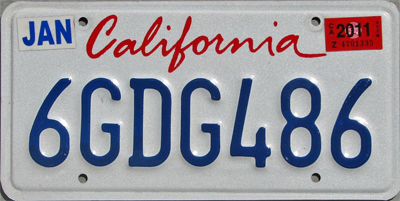
\includegraphics[scale=.4]{California}
\end{center}
\end{multicols}
\begin{solution}{\vfill}
$10\cdot 26\cdot 26\cdot 26\cdot 10\cdot 10\cdot 10=26^3\cdot 10^4
=175,760,000$
\end{solution}
\newpage

\question[16] Two cards are drawn at random from a deck of playing cards
without replacement.
\begin{parts}
\part What is the probability that the second card is a Queen
given that the first card is a Queen?
\begin{solution}[1in]
$\frac{3}{51}\approx 0.059$
\end{solution}
\part What is the probability that both cards are Queens?
\begin{solution}[1in]
$\frac{4}{52}\cdot\frac{3}{51}=\frac{1}{221}
\approx 0.005$
\end{solution}
\end{parts}

\question[18] The following table lists
the languages other than English spoken by residents
of Iowa between 2008 and 2012, organized by the age
of the resident.\footnote{Source: {\tt www.census.gov}}
\[\begin{array}{r|rrr|r}
\text{Language}&\text{$5$--$17$}
&\text{$18$--$64$}&\ge 65&\text{Total}\\\hline
\text{Spanish or Spanish Creole}&32,196&75,674&4,114&111,984\\
\text{Other Indo-European}&8,978&29,811&6,530&45,319\\
\text{Asian or Pacific Island}&5,624&27,022&2,255&34,901\\
\text{Other}&2,386&7,874&423&10,683\\\hline
\text{Total}&49,184&140,381&13,322&202,887
\end{array}\]
\begin{parts}
\part What is the probability that a randomly selected
resident spoke Spanish or Spanish Creole
given that that individual was between $65$ years old or older?
\begin{solution}[2cm]
$\frac{4114}{13322}\approx 0.309$
\end{solution}
\part What is the probability that a randomly selected
resident that spoke a language other than English
was between $18$ and $64$ years old?
\begin{solution}[2cm]
$\frac{140381}{202887}\approx 0.692$
\end{solution}
\part How many residents of age $65$ or older
spoke a language other than English?
\begin{solution}[2cm]
$13,322$
\end{solution}
\end{parts}
\newpage

\question[24] In a recent survey of 884 Americans between the ages
of $18$ and $50$, $120$ reported that they have tattoos,
$72$ have body piercings, and $41$ have both.
\footnote{2004, American Journal of Dermatology}

\begin{parts}
\part What is the probability that a randomly
selected American has a tattoo?
\begin{solution}[1.5cm]
$\frac{120}{884}\approx 0.136$
\end{solution}
\part What is the probability that a randomly
selected American has a piercing?
\begin{solution}[1.5cm]
$\frac{72}{884}\approx 0.081$
\end{solution}
\part What is the probability that a randomly
selected American has a both a tattoo and a piercing?
\begin{solution}[1.5cm]
$\frac{41}{884}\approx 0.056$
\end{solution}
\part\label{Independent} According to this data do
the decision to get a piercing and the decision
to get a tattoo appear to be independent?
\begin{solution}[1.5cm]
No, since $0.136\cdot 0.081\approx 0.011\ne 0.056$
\end{solution}
\part Does your response to part~(\ref{Independent}) make
sense in the context of the problem?
\begin{solution}[1.5cm]
We'll accept anything along the lines of people with
tattos being more inclinded to get piercings or vice versa.
\end{solution}
\part What is the probability that a randomly
selected American has a tattoo given that that individual
has a piercing?
\begin{solution}[1.5cm]
$\begin{xy}<.5cm,0cm>:
(-1,2)*+!D{\text{T}};
(1,2)*+!D{\text{P}};
(-1,0)*\cir<1cm>{};
(1,0)*\cir<1cm>{};
(0,0)*{41};
(-2,0)*{79};
(2,0)*{31};
(4,0)*{733};
\end{xy}$
\qquad $\frac{41}{72}\approx 0.569$
\end{solution}
\part What is the probability that a randomly
selected American has a piercing given that that individual
does {\bf not} have a tattoo?
\begin{solution}[1.5cm]
$\frac{31}{31+733}\approx 0.041$
\end{solution}
\end{parts}
\newpage

\question[16] How many anagrams of the word
\textsf{Tintinnabulation} are there?
\begin{solution}[3in]
The number of times each distinct letter appears is
shown in the following table.
\[\begin{array}{r|cccccccc}
\text{letter}&a&b&i&l&n&o&t&u\\\hline
\text{frequency}&2&1&3&1&4&1&3&1
\end{array}\]
Thus the number of anagrams is
\[\frac{16!}{2!3!4!3!}=12,108,096,000.\]
\end{solution}

\question[16] Suppose $E=\left\{r,t,u,v,w\right\}$,
$F=\left\{s,t,x,y,z\right\}$, and $G=\left\{r,s,v,y,z\right\}$.
\begin{parts}
\part Calculate $\left(E\cup G\right)\cap\left(F\cup G\right)$
\begin{solution}[1.5in]
\begin{align*}
E\cup G&=\left\{r,s,t,u,v,w,y,z\right\}\\
F\cup G&=\left\{r,s,t,v,x,y,z\right\}\\
\text{so}\quad
\left(E\cup G\right)\cap\left(F\cup G\right)
&=\left\{r,s,t,v,y,z\right\}\\
\end{align*}
\end{solution}
\part Calculate $\left(E\cap F\right)\cup G$
\begin{solution}
\begin{align*}
E\cap F&=\left\{t\right\}\\
\text{so}\quad\left(E\cap F\right)\cup G
&=\left\{r,s,t,v,y,z\right\}
\end{align*}
\end{solution}
\end{parts}

\vfill
\begin{center}\gradetable[h][questions]\end{center}

\end{questions}
\end{document}
